This calculator computes loss maps and loss statistics due to a single seismic
event, for a collection of assets. The hazard input can be a single ground
motion field (e.g. the median distribution of ground motion in the region of
interest) or a set of ground motion fields allowing the characterisation of
the inter- and intra-event variability from the GMPE. It is noted that the
hazard input can either be calculated using the hazard component of OpenQuake-
engine (oq-hazardlib), or provided to the risk component iian external file
following the respective Natural hazards' Risk Markup Language (NRML) schema
(see \href{http://github.com/gem/oq-nrmllib}{oq-nrmllib}). A vulnerability
model is combined with the distribution of the ground motions at each asset
location to calculate the loss distribution for each asset, as well as the
statistics of the total loss throughout the region of interest. The required
input files and resulting output files are depicted in
Figure~\ref{fig:io-structure-scenario-risk}.

\begin{figure}[ht]
\centering
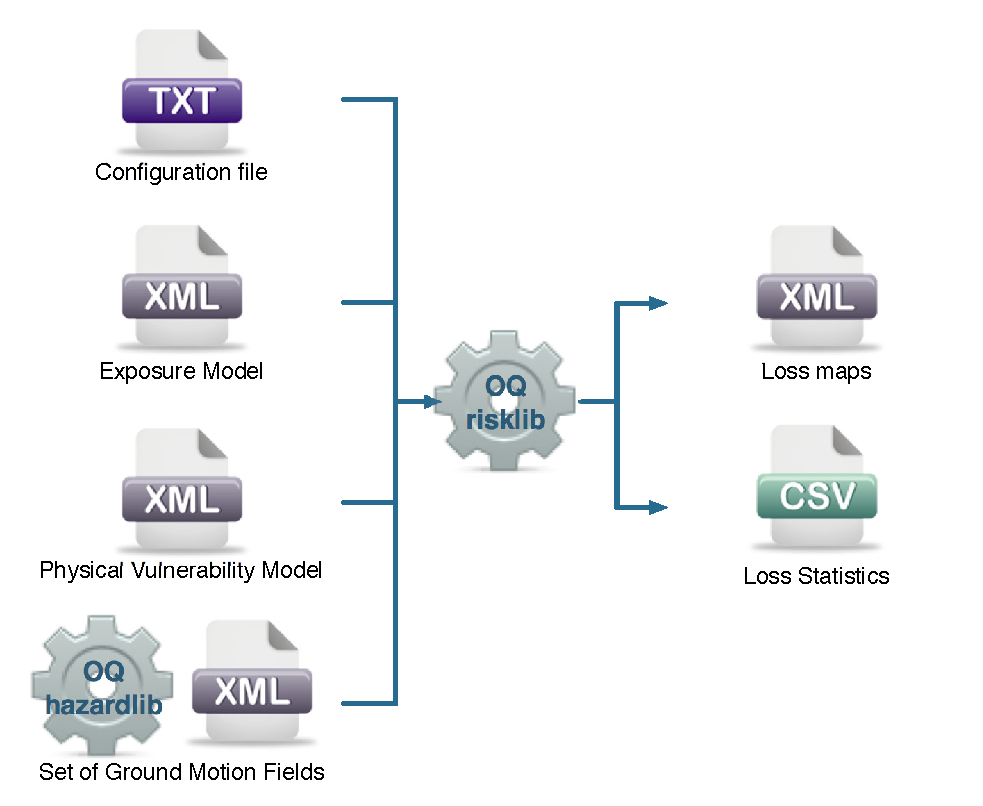
\includegraphics[width=9cm,height=7cm]{figures/risk/io-structure-scenario-risk.pdf}
\caption{Scenario Risk Calculator input/output structure.}
\label{fig:io-structure-scenario-risk}
\end{figure}